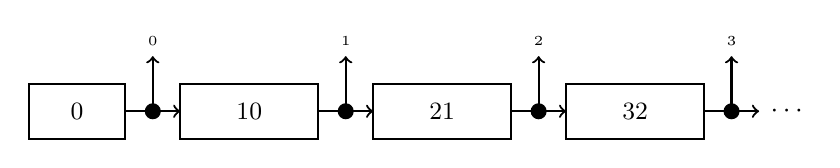
\begin{tikzpicture}[scale=0.35,thick] % , baseline = -3.5pt


\draw (-3.5,-1) rectangle (0, 1);
\node[anchor=center] (text) at (-1.75,0) {\small $\probof{\catvariableof{0}}$};
\draw[->] (0,0) -- (2,0);
\draw[fill] (1,0) circle (0.25cm);
\draw[->] (1,0) -- (1,2) node[above] {\tiny $\catvariableof{0}$};
\draw (2,-1) rectangle (7, 1);
\node[anchor=center] (text) at (4.5,0) {\small $\condprobof{\catvariableof{1}}{\catvariableof{0}}$};
\draw[->]  (7,0) -- (9,0);
\draw[fill] (8,0) circle (0.25cm);
\draw[->] (8,0) -- (8,2) node[above] {\tiny $\catvariableof{1}$};
\draw (9,-1) rectangle (14, 1);
\node[anchor=center] (text) at (11.5,0) {\small $\condprobof{\catvariableof{2}}{\catvariableof{1}}$};
\draw[->]  (14,0) -- (16,0);
\draw[fill] (15,0) circle (0.25cm);
\draw[->] (15,0) -- (15,2) node[above] {\tiny $\catvariableof{2}$};
\draw (16,-1) rectangle (21, 1);
\node[anchor=center] (text) at (18.5,0) {\small $\condprobof{\catvariableof{3}}{\catvariableof{2}}$};
\draw[->]  (21,0) -- (23,0);
\draw[fill] (22,0) circle (0.25cm);
\draw[->] (22,0) -- (22,2) node[above] {\tiny $\catvariableof{3}$};
\node[anchor=center] (text) at (24,0) {$\cdots$};

\end{tikzpicture} 